\chapter{Expected Result}

The proposed Universal Turing Machine (UTM) is expected to closely resemble Mike Davey's Turing Machine in form and functionality but will feature several key improvements and innovations aimed at enhancing its usability, versatility, and educational value \cite{davey2010}. Mike Davey's "A Turing Machine" is widely regarded as a foundational demonstration of Turing's theoretical principles in physical form. Its design effectively captures the essential components of a Turing Machine, including the tape, read/write heads, and control mechanisms. However, the proposed UTM aims to build upon this foundation by addressing certain limitations and introducing features, such as:
\begin{itemize}
    \item \textbf{Punched Card Programming:} Unlike Davey's machine, the proposed UTM will utilize punched cards for programming. This allows for a more user-friendly and modular way of defining state transition tables and algorithms, simplifying the process of reprogramming the machine for different tasks.
    \item \textbf{Improved Hardware Design:} By integrating modern components such as stepper motors, servo motors, and IR sensors, the hardware will provide higher precision, reliability, and flexibility. The control system, based on Arduino and ESP32-CAM, ensures seamless coordination of all mechanical and computational operations.
    \item \textbf{Educational Utility:} The proposed design emphasizes accessibility for educational purposes. Features such as the paper-programmable interface, LCD display, intuitive control panel, and a digital simulation (tlang) complement the physical machine to aid understanding of Turing's concepts.
\end{itemize}

\begin{figure}[h!]
    \centering
    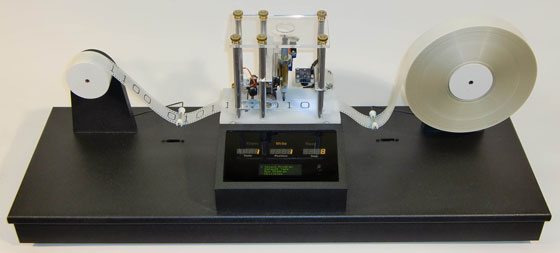
\includegraphics[width=0.9\textwidth]{content/images/mikeDavey.jpg}
    \caption{Mike Davey's "A Turing Machine"}
    \label{fig:expectedOutcome}
\end{figure}


\begin{figure}[h!]
    \centering
    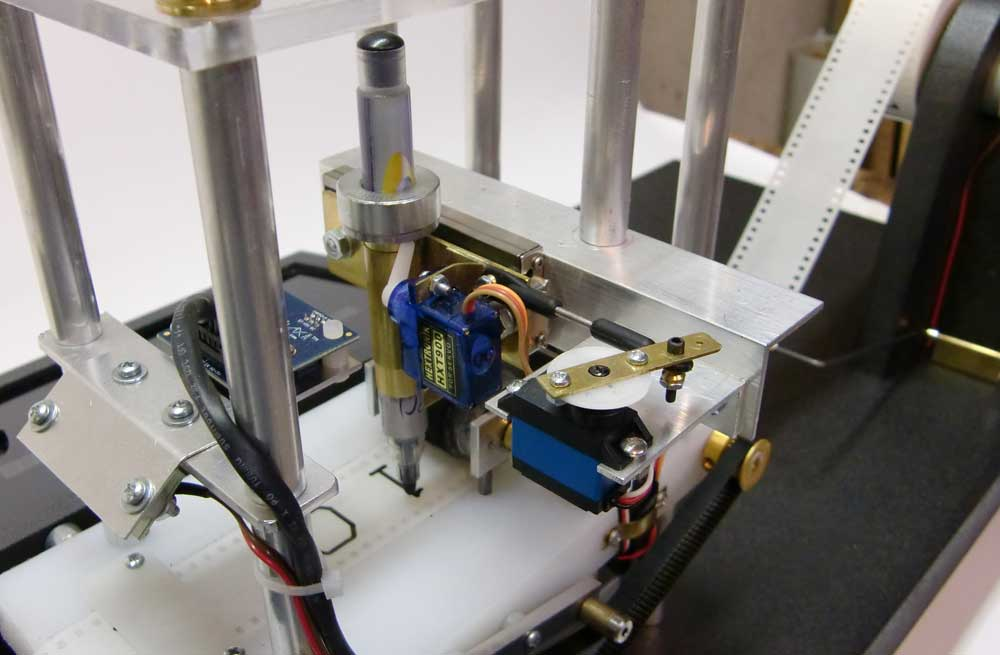
\includegraphics[width=0.7\textwidth]{content/images/mikeDaveyRW.jpg}
    \caption{Mike Davey’s Read/Write Head}
    \label{fig:mikeDaveyRW}
\end{figure}

Figure \ref{fig:expectedOutcome} illustrates the physical design of Mike Davey's Turing Machine, which serves as an inspiration for this project. While the proposed UTM shares a similar conceptual framework, the above-mentioned enhancements are expected to elevate its practical utility and user experience. The completed UTM will not only demonstrate Turing's theoretical concepts in hardware but also provide a platform for practical experimentation with algorithms, computational logic, and the principles of discrete mathematics. It is expected to serve as a valuable educational tool, as well as a proof-of-concept for bridging theoretical computation with real-world applications.

Figure \ref{fig:mikeDaveyRW} illustrates Mike Davey’s Turing Machines's read/write head, which forms a critical part of the machine’s operation. The proposed UTM’s read/write head is expected to work in a similar manner with two servos moving the writing mechanism in two axes. However, the proposed design introduces several enhancements aimed at improving precision, reliability, and versatility. The proposed UTM will employ an infrared (IR) sensor for symbol detection on the tape, ensuring accurate readings under various lighting conditions. Writing and erasing operations will be facilitated by a servo motor-driven mechanism, allowing precise symbol placement and modification. Additionally, the hardware will include a more robust tracking system for the tape position, reducing mechanical drift and improving overall operational accuracy.

In conclusion, while inspired by Mike Davey’s pioneering work, the proposed UTM seeks to extend the capabilities of its predecessor. By integrating advanced hardware components and user-friendly features such as punched card programming and a complementary digital simulation, the UTM aims to provide a comprehensive educational and research platform that bridges the gap between theoretical and applied computational science.







